%!TEX root = ../thesis.tex


% **************************** Define Graphics Path **************************
\ifpdf
    \graphicspath{{Chapter3/Figs/Raster/}{Chapter3/Figs/PDF/}{Chapter3/Figs/}{Chapter3/BSIQPE/}}
\else
    \graphicspath{{Chapter3/Figs/Vector/}{Chapter3/Figs/}{Chapter3/BSIQPE/}}
\fi

\section{Boosting Quantum Phase Estimation with arbitary ancilla states}
\label{section:boostedphaseestimation}

\subsection{Introduction}
Standard methods \cite{babbush2018encoding, rendon2022effects, berry2024analyzing, greenaway2024case, patel2026optimal} for coherently boosting QPE rely upon choosing specific input ancillary states. They perform QPE using ancillas initialised to the state $\frac{1}{\sqrt{N}}\sum_x \alpha(x) \ket{x}$ for some window function $\alpha(x)$ instead of the standard uniform superposition, such that the output amplitudes are given by $\hat\alpha$, the discrete Fourier transform of $\alpha(x)$ (Eq.~\eqref{eq:windowed_qpe}). By choosing $\alpha$ to be a window function one can ensure that $\hat \alpha$ is narrowly peaked, thus QPE is boosted. Unfortunately, this is not sufficient for algorithms which coherently encode an energy estimate in an ancilla register and then reuse this register without resetting it, as the protocol must work even when the register is not initialised to $\ket{0}$. For example, the rewinding procedure of the quantum Metropolis algorithm (Chapter~\ref{chapter:quantum_metropolis}) requires exactly this. In addition to being boosted, such algorithms require QPE to be ``shift-invariant": starting from a register value $p$ rather than zero simply translates the output by $p$. Thus, such algorithms depend upon a ``boosted shift-invariant" quantum phase estimation protocol that applies a shift to an ancilla register within a given bound of the true energy (with $\tilde E_j = \frac{N}{2\pi}E_j$ with $N=2^{\eta}$ for an $\eta$ ancilla energy register):
\begin{equation}
  \ket{\psi_j}\ket{p} \;\mapsto\; \sum_{s} \alpha(E_j,s)\,\ket{\psi_j}\ket{p+s},\qquad \alpha(E_j,s) = 0 \ \text{ for } |s-\tilde E_j|_{N} > \mu .
  \label{eq:bsi_shift_invariant_qpe}
\end{equation}
where $\ket{\psi_j}$ is an energy eigenstate with energy $E_j$, $\mu$ is the allowed error in register units, and $|\cdot|_{N}$ measures distance accounting for the register's wraparound. However, Appendix H of \cite{chen2023quantumthermalstatepreparation} proved it is impossible to implement any unitary approximating this ``boosted shift-invariant" quantum phase estimation protocol \eqref{eq:bsi_shift_invariant_qpe}.

Our Boosted State-Independent Quantum Phase Estimation (BSI-QPE) protocol navigates around this no-go theorem, achieving coherent boosting without requiring a specially prepared input ancilla state. It ensures the magnitude of the shift in the ancilla register is close to the true energy with the sign of this shift recorded in an additional flag qubit:
\begin{equation}
  \ket{\psi_j}\ket{p}\ket{f} \;\mapsto\; \sum_{s,f'} \alpha_{f'f}(E_j,s)\,
  \ket{\psi_j}\ket{p+(-1)^{f'}s}\ket{f'},
  \qquad \sum_{|s-\tilde E_j|_{N} > \mu} \big|\alpha_{f'f}(E_j,s)\big| = O(e^{-\nu\mu}),
  \label{eq:bsi_qpe}
\end{equation}
for some $\nu > 0$ determined by the choice of window functions (Section~\ref{section:appendix}). This action is illustrated in Fig.~\ref{fig:Gshift}. This protocol is implementable and can fulfil the same role as the impossible protocol \eqref{eq:bsi_shift_invariant_qpe}, with the modification that whenever we previously controlled off the value of the energy register we now must also control off the flag qubit.

\subsection{Boosted State-Independent Quantum Phase Estimation}
\begin{figure*}
\centering
\begin{tikzpicture}
 
% ---- parameters -------------------------------------------------
\def\qq{5.6}        % input value q
\def\dd{3.6}        % shift  (2^eta/2pi) E_j t
\def\sg{0.42}       % peak width
\def\mw{1.25}       % half-window mu
\def\hh{2.6}        % peak height
\pgfmathsetmacro{\cL}{\qq-\dd}
\pgfmathsetmacro{\cR}{\qq+\dd}
 
% ---- axes -------------------------------------------------------
\draw[<->,thick] (-1,0) -- (12.6,0);
\node[anchor=west,font=\small] at (11.0,0.42) {output energy register};
% \draw[->,thick] (0.4,-0.05) -- (0.4,4.1) node[above,font=\small] {amplitude};
 
% ---- input value q ---------------------------------------------
% \draw[->, thick] (\qq,0) -- (\qq,4.1);
\node[gray!40!black,below,font=\small] at (\qq,-0.06) {$q$};
\draw[->,thick] (\qq,0) -- (\qq,4.1) node[above,font=\small] {amplitude magnitude};

 
% ---- one output branch ------------------------------------------
% #1 centre  #2 colour  #3 F-label  #4 centre label
\newcommand{\branch}[4]{%
  \fill[#2!10] (#1-\mw,0) rectangle (#1+\mw,2.95);
  \draw[#2!35,dashed] (#1-\mw,0) -- (#1-\mw,2.95);
  \draw[#2!35,dashed] (#1+\mw,0) -- (#1+\mw,2.95);
  \begin{scope}
    \clip (0.45,-0.05) rectangle (11.3,4.0);
    \draw[#2,line width=1pt] plot[domain=#1-3.0:#1+3.0,samples=240,smooth]
        (\x,{\hh*exp(-(\x-#1)*(\x-#1)/(2*\sg*\sg))});
  \end{scope}
  \draw[#2!55,densely dotted] (#1,0) -- (#1,\hh+0.1);
  \node[#2!75!black,font=\small] at (#1,3.75) {#3};
  \draw[<->,#2!70!black,line width=0.7pt]
        (#1-\mw,-0.3) -- (#1+\mw,-0.3) node[midway,below=4pt,font=\small] {$2\mu$};
  % \node[#2!75!black,font=\small] at (#1,-1.5) {#4};
}
 
\branch{\cL}{red!70!black}{$F=\ket{1}$ afterwards}{$q-\frac{N}{2\pi}E_j t$}
\branch{\cR}{blue!65!black}{$F=\ket{0}$ afterwards}{$q+\frac{N}{2\pi}E_j t$}
 
% ---- shift arrows ----------------------------------------------
\draw[<-,thick,red!70!black]  (\cL+0.1,3.15) -- (\qq-0.1,3.15)
      node[midway,above,font=\small] {$-\frac{N}{2\pi}E_j t$};
\draw[->,thick,blue!65!black] (\qq+0.1,3.15) -- (\cR-0.1,3.15)
      node[midway,above,font=\small] {$+\frac{N}{2\pi}E_j t$};
 
% ---- tail annotation -------------------------------------------
% \node[gray!55!black,align=center,font=\scriptsize] at (\qq,1.15)
%       {exponentially\\ suppressed tails};
% \draw[gray!55!black,->,shorten >=2pt] (\qq-1.0,0.95) -- (\cL+1.65,0.13);
% \draw[gray!55!black,->,shorten >=2pt] (\qq+1.0,0.95) -- (\cR-1.65,0.13);
 
\end{tikzpicture}
\caption{Action of BSI-QPE on an energy eigenstate $\ket{\psi_j}$ with the energy register initially holding $q$. The output has two branches centered on $q\pm\frac{N}{2\pi}E_jt$, distinguished by the output flag qubit $F$. The window functions concentrate the amplitudes around these centres and suppress the tails exponentially. The exact shape of the amplitude distribution depends upon the value of $F$ before the action of BSI-QPE, however it is of little consequence as they both have exponentially decaying tails.}
\label{fig:Gshift}
\end{figure*}

Our construction uses two window functions $\alpha(x)$ and $\beta(x) = \sqrt{1-\alpha(x)^2}$ (for $x\in\{0,1,\ldots,N-1\}$) which are both narrowly peaked in the Fourier domain. We introduce these windows via the following multi-controlled single-qubit rotation:
\begin{equation}
   CR_Y = \sum_k \ket{k}\bra{k}\otimes \begin{pmatrix}
        \alpha(k)& \beta(k)\\
        -\beta(k)& \alpha(k)
    \end{pmatrix}
\end{equation}

We also require the following time evolution gadget which is constructed as shown in Fig~\ref{fig:CRZ}:
\begin{equation}
    CR_Z =\sum_{j,k}\ket{\psi_j}\bra{\psi_j}\otimes\ket{k}\bra{k} \otimes \begin{pmatrix}
        e^{\frac{iE_jkt}{2}}&0\\
        0 & e^{-\frac{iE_jkt}{2}}
    \end{pmatrix}
\end{equation}
\begin{figure*}
    \centering
\begin{center}$
\vcenter{\hbox{
\resizebox{!}{2.5cm}{
\begin{tikzpicture}
\begin{yquant*}
qubit {$\ket{\psi_j}$} s;
init {$R$ ($\eta$ ancillas)} (a[0,1],ellipsis, aend);
slash s;
hspace {0.1cm} -;
discard ellipsis;
% qubit {} aend;
qubit {$F$} f;
box {$CR_Z$} (s,a,ellipsis, aend, f);
% text {$\ket{0}$} f;
\end{yquant*}
\end{tikzpicture}}}}
=
\vcenter{\hbox{
\resizebox{!}{2.5cm}{
    \begin{tikzpicture}
\begin{yquant*}
qubit {$\ket{\psi_j}$} s;
init {$R$} (a[0,1],ellipsis, aend);
discard ellipsis;
% qubit {} aend;
qubit {$F$} f;
slash s;
hspace {0.1cm} -;
box {$U^{\dagger 2^0}$} (s) | a[0], f;
box {$U^{\dagger 2^1}$} (s) | a[1], f;
hspace {0mm} -;
dots ellipsis;
box {$U^{\dagger 2^{\eta-1}}$} (s) | aend[0], f;
box {$U^{2^0}$} (s) | a[0]~ f;
box {$U^{ 2^1}$} (s) | a[1]~ f;
hspace {0mm} -;
dots ellipsis;
box {$U^{ 2^{\eta-1}}$} (s) | aend[0]~ f;
\end{yquant*}
\end{tikzpicture}}}}
$\end{center}
\caption{Quantum circuit for implementing an $Z$ rotation on an ancilla qubit that is dependent upon the energy of the system. The unitary $U=e^{\frac{iHt}{2}}$ is implemented through some quantum time evolution algorithm (e.g. trotterisation \cite{lloyd1996universal}, qubitization \cite{Low2019hamiltonian}) up to an operator norm error of $\epsilon^T_t$. Throughout this work we assume  $\epsilon^T_t$ is negligible, and use perfect quantum time evolution in our error analysis.}
    \label{fig:CRZ}
\end{figure*}
Conditioned on the system being in $\ket{\psi_j}$ and the ancilla register in $\ket{k}$,
both gadgets act on the flag qubit $F$ as single-qubit rotations: $CR_Y$ applies
$R_Y[2\arccos\alpha(k)]$ and $CR_Z$ applies $R_Z[E_jkt]$, where throughout we use the convention
\begin{align}
R_Z(\phi) = \begin{pmatrix} e^{i\phi/2} & 0\\ 0 & e^{-i\phi/2}\end{pmatrix}\\
R_Y(\theta) = \begin{pmatrix} \cos\frac{\theta}{2} & \sin\frac{\theta}{2}\\ -\sin\frac{\theta}{2} & \cos\frac{\theta}{2}\end{pmatrix}
\end{align}
\begin{figure*}
    \centering
\begin{center}$
\vcenter{\hbox{
\resizebox{!}{2.5cm}{
\begin{tikzpicture}
    \begin{yquant*}
qubit {$\ket{\psi_j}$} s;
init {$R$ ($\eta$ ancillas)} (a[0,1],ellipsis, aend);
slash s;
% hspace {0.1cm} -;
discard ellipsis;
% qubit {} aend;
qubit {$F$} f;
dots ellipsis;
box {BSI-\\QPE} (s,a,ellipsis, aend, f);
% text {$\ket{0}$} f;
\end{yquant*}
\end{tikzpicture} }}}
=
\vcenter{\hbox{
\resizebox{!}{3cm}{
\begin{tikzpicture}
    \begin{yquant*}
qubit {$\ket{\psi_j}$} s;
init {$R$} (a[0,1],ellipsis, aend);
slash s;
discard ellipsis;
% qubit {} aend;
qubit {$F$} f;
dots ellipsis;
box {QFT} (a,ellipsis, aend);
[this subcircuit box style={dashed, "$R_Z[E_jt(k-k')]$"}]
subcircuit {
qubit {} s;
qubit {} a[2];
nobit ellipsis;
qubit {} aend;
qubit {} f;
% dots ellipsis;
box {$CR_Z$} (s,a,ellipsis, aend, f);
x aend[0];
dots ellipsis;
box {$CR_Z^{\dagger}$} (s,a,ellipsis, aend, f);
x aend[0];
dots ellipsis;
} (s,a,ellipsis, aend, f);
box {$CR_Y$} (a,ellipsis, aend, f);
[this subcircuit box style={dashed, "$R_Z[E_jt(k+k'-N)]$"}]
subcircuit {
qubit {} s;
qubit {} a[2];
nobit ellipsis;
qubit {} aend;
qubit {} f;
box {$CR_Z$} (s,a,ellipsis, aend, f);
x aend[0];
dots ellipsis;
box {$CR_Z$} (s,a,ellipsis, aend, f);
x aend[0];
dots ellipsis;
box {$U^{\dagger N}$} (s) ~ f;
box {$U^{N}$} (s) | f;
} (s,a,ellipsis, aend, f);
box {iQFT} (a,ellipsis, aend);
% text {$\ket{0}$} f;
\end{yquant*}
\end{tikzpicture} }}}
$\end{center}

\caption{Quantum circuit implementing boosted state-independent quantum phase estimation (BSI-QPE). We highlight how the combinations of $CR_Z$ and $X$ gates operators correspond to the single qubit $R_Z$ given in Eq.~\ref{eq:euler} with $k$ being the value stored in the $\eta$ ancillas and $k' = k + \frac{N}{2} \mod N$}
\label{fig:circuit}
\end{figure*}
\begin{figure*}
    \centering
\begin{tikzpicture}
    \begin{yquant*}
qubit {$\ket{\psi_j}$} s;

init {$\eta$ ancillas} (a[0,1],ellipsis, aend);
slash s;
discard ellipsis;
% qubit {} aend;
dots ellipsis;
box {QFT} (a,ellipsis, aend);

box {$U^{ 2^1}$} (s) | a[0];
box {$U^{ 2^2}$} (s) | a[1];
hspace {0mm} -;
dots ellipsis;

box {$U^{ N}$} (s) | aend[0];
box {$U^{\dagger N}$} (s);
box {iQFT} (a,ellipsis, aend);

% text {$\ket{0}$} f;
\end{yquant*}
\end{tikzpicture} 

\caption{Quantum circuit implementing unboosted state-independent QPE with $U=e^{\frac{iHt}{2}}$, equivalent to choosing $\alpha(x)=1$ for BSI-QPE and acting upon $\ket{0}_F$. This slightly differs from the standard formulation of QPE \cite{Nielsen_Chuang_2010} by beginning with $QFT$ rather than $H^{\otimes \eta}$ and the addition of $U^{\dagger N}$ at the end. }
\label{fig:standard_qpe}
\end{figure*}
% \begin{widetext}
BSI-QPE is built from the $R_ZR_YR_Z$ (Euler) decomposition of a single-qubit unitary~\cite{Nielsen_Chuang_2010}, which in the convention above reads
\begin{equation}
\label{eq:euler}
R_Z(\phi_1)R_Y(\theta)R_Z(\phi_2) = \begin{pmatrix}
\cos\frac{\theta}{2}\,e^{i(\phi_1+\phi_2)/2} & \sin\frac{\theta}{2}\,e^{i(\phi_1-\phi_2)/2}\\
-\sin\frac{\theta}{2}\,e^{-i(\phi_1-\phi_2)/2} & \cos\frac{\theta}{2}\,e^{-i(\phi_1+\phi_2)/2}
\end{pmatrix}.
\end{equation}
The circuit in Fig.~\ref{fig:circuit} implements this with angles that depend on the ancilla value $k$. The $X$ gates on the last ancilla qubit map $k\to k' = k+\frac{N}{2} \bmod N$, so the first dashed block implements $R_Z[E_jt(k-k')]$ and the second implements $R_Z[E_jt(k+k'-N)]$, where the $-N$ comes from the $F$-controlled $U^{\pm N}$. Substituting
\begin{equation}
\label{eq:angles}
\theta = 2\arccos\alpha(k),\qquad \phi_1 = E_jt(k+k'-N),\qquad \phi_2 = E_jt(k-k')
\end{equation}
into Eq.~\eqref{eq:euler}, and using $\cos\frac{\theta}{2}=\alpha(k)$, $\sin\frac{\theta}{2}=\beta(k)$, gives
\begin{equation}
\begin{pmatrix}
\alpha(k)e^{iE_jtk}e^{-\frac{iE_jtN}{2}} & \beta(k)e^{iE_jt k'}e^{-\frac{iE_jtN}{2}}\\
-\beta(k)e^{-iE_jt k'}e^{\frac{iE_jtN}{2}} & \alpha(k)e^{-iE_jtk}e^{\frac{iE_jtN}{2}}
\end{pmatrix}.
\end{equation}
Hence, summing over $k$ and the QFTs, we get the following operation:
\begin{multline}
        \text{BSI-QPE} = \frac{1}{N}\sum_j\sum_{p,q,k} \begin{pmatrix}
        \alpha(k)e^{iE_jtk}e^{-\frac{iE_jtN}{2}} && \beta(k)e^{iE_jt[(k+\frac{N}{2})\text{mod} N]}e^{-\frac{iE_jtN}{2}}\\
        -\beta (k)e^{-iE_jt[(k+\frac{N}{2})\text{mod} N]}e^{\frac{iE_jtN}{2}} && \alpha(k)e^{-iE_jtk}e^{\frac{iE_jtN}{2}}
    \end{pmatrix}e^{\frac{2\pi i}{N}k(q-p)} \\\otimes\ket{p}\bra{q}\otimes\ket{\psi_j}\bra{\psi_j}
\end{multline}
This can be simplified to:
\begin{equation}
    \text{BSI-QPE} = \sum_j\sum_{p,q} \begin{pmatrix}
        (-1)^{q-p}\hat\alpha(q-p+\frac{N}{2\pi}E_jt) && \hat\beta(q-p+\frac{N}{2\pi}E_jt)\\
        -\hat\beta (q-p-\frac{N}{2\pi}E_jt) && (-1)^{q-p}\hat\alpha(q-p-\frac{N}{2\pi}E_jt)
    \end{pmatrix}\otimes\ket{p}\bra{q}\otimes\ket{\psi_j}\bra{\psi_j}
\end{equation}
% \begin{multline}
%   \sum_j \sum^{N}_{p,q} \hat \alpha(p - q - \frac{N t}{2\pi}E_j)\ket{0}\bra{0} \otimes\ket{p}\bra{q} \otimes \ket{\psi_j} \bra{\psi_j}\\
%   + \ket{0}\bra{0} \otimes\bm{\varepsilon}^T_{kt}
% \end{multline}
where $\hat \alpha$ is the discrete Fourier transform of $\alpha$ as given by:
\begin{equation}
   \hat\alpha(x) =\frac{1}{N}\sum_{k=-\frac{N}{2}}^{\frac{N}{2}-1} \alpha(k+\frac{N}{2})e^{\frac{2\pi i}{N}xk}
\end{equation}
and $\hat \beta$ is the discrete Fourier transform of $\beta$ given by:
\begin{equation}
    \hat\beta(x) =\frac{1}{N}\sum_{k=-\frac{N}{2}}^{\frac{N}{2}-1} \beta(k)e^{\frac{2\pi i}{N}kx}
\end{equation}
 where $\beta(k)$ is extended by $\beta(k) = \beta(k \mod N)$. 
 \begin{remark}[Why the Fourier transforms use different origins]
     The definition of $\hat\alpha$ shifts the window $\alpha$ by half a period, whereas the definition of $\hat\beta$ does not. This allows each window to be small at the boundaries of its own Fourier summation interval. Using the same origin for both would prevent this, because $\alpha^2+\beta^2=1$. For off-grid energies, the resulting boundary mismatch would introduce slowly decaying tails. The different origins are therefore essential to obtaining exponential tail suppression for both branches.
 \end{remark}
Throughout the rest of this thesis, we will use the following notational shorthand: 
\begin{equation}
    G_j^{pq} = \begin{pmatrix}
        (-1)^{q-p}\hat\alpha(q-p+\frac{N}{2\pi}E_jt) && \hat\beta(q-p+\frac{N}{2\pi}E_jt)\\
        -\hat\beta (q-p-\frac{N}{2\pi}E_jt) && (-1)^{q-p}\hat\alpha(q-p-\frac{N}{2\pi}E_jt)
    \end{pmatrix}
\end{equation}
This shows that BSI-QPE shifts the energy-index register by approximately $\frac{N}{2\pi}E_jt$, in a direction given by the qubit $F$ after the application as demonstrated by Fig.~\ref{fig:Gshift}. 

% \end{widetext}
\medskip
\noindent\fbox{%
\begin{minipage}{\dimexpr\columnwidth-2\fboxsep-2\fboxrule\relax}
\textbf{Summary of BSI-QPE}

BSI-QPE shifts the value stored in the energy register by approximately the magnitude of the system's energy, with the sign of the shift recorded in the flag qubit $F$. Hence, for an $\eta$-qubit register initially holding $q$ the output amplitudes are concentrated around
\begin{equation}
\begin{aligned}
q+\frac{N}{2\pi}E_jt
    &\quad\text{for }F=\ket{0},\\
q-\frac{N}{2\pi}E_jt
    &\quad\text{for }F=\ket{1}.
\end{aligned}
\end{equation}
where the arithmetic is modulo $N$. Figure~\ref{fig:Gshift} illustrates this action.\\

Using the window functions constructed in Section~\ref{section:appendix}, both branches have exponentially suppressed tails. Changing $q$ simply translates the output, and no specially prepared initial state of the energy register or flag qubit is required. The energy eigenstate $\ket{\psi_j}$ is unchanged. 
\end{minipage}%
}\medskip
\subsection{Complementary Window functions}
\label{section:appendix}
BSI-QPE places unusual demands upon its window functions. Rather than a single window function with a rapidly decaying Fourier transform, BSI-QPE requires a pair of window functions $\alpha(x), \beta(x)$ which must satisfy the following characteristics for all $x \in \mathbb{R}$:
\begin{enumerate}
    \item $\alpha(x)^2+\beta(x)^2 =1$
    \item $\alpha(x+N) = \alpha(x)$ and $\beta(x+N) = \beta(x)$
    \item $\sum_{|k|_{N}\geq\mu}|\hat \alpha(k)|, \sum_{|k|_{N}\geq\mu}|\hat \beta(k)| \leq \epsilon_\Delta$ with $\epsilon_\Delta = O(\frac{1}{\nu}e^{-\nu\mu})$ for some $\nu > 0$
\end{enumerate}
The first characteristic ensures that $CR_Y$ is unitary, and is a strong constraint: wherever $\alpha$ is small $\beta$ must be close to one, and vice versa. None of the standard window functions (e.g. DPSS, Kaiser window, Gaussian) are close to satisfying this form. Taking $\beta = \sqrt{1-\alpha^2}$ for a standard window function $\alpha$ typically produces a kink where $\alpha$ reaches its maximum, and hence the Fourier transform of $\beta$ only decays polynomially. Therefore, we must design a novel pair of window functions. In this work we have chosen $\alpha(x) = \text{sech}( r\cos^{2b} \frac{\pi x}{N})$ and $\beta(x) = \text{tanh}(r \cos^{2b} \frac{\pi x}{N})$ for $b \in \mathbb{Z}_{>0}$ and $r \in \mathbb{R}^+$. These satisfy characteristics 1 and 2 directly. Below we demonstrate analytically and numerically that they satisfy characteristic 3.

\begin{lemma}
    For every positive integer $b$ and $0 < r \leq \pi2^{b-1}$ we have that $\alpha(x)= \text{sech}( r\cos^{2b} \frac{\pi x}{N})$ and $\beta(x) = \text{tanh}(r \cos^{2b} \frac{\pi x}{N})$ are analytic and satisfy $|\alpha(x)|, |\beta(x)| \leq 2$ in the closed strip $| \operatorname{Im} z| \leq \frac{N\nu}{2\pi}$ for all $0 < \nu \leq \frac{1}{2b}$. 
    \label{lemma:appendixc}
\end{lemma}
\begin{proof}
    Let $u + iv = \frac{\pi z}{N}$, $\zeta = \cos (u+iv)$ and $w = r \zeta^{2b}$. Let us consider the imaginary part of $\zeta$:
    \begin{equation}
        |\operatorname{Im} \zeta |  = | \sin u \sinh v | \leq \sinh |v|  \leq \sinh \frac{1}{4b}
    \end{equation}
    If we bound $|\zeta|$ away from $0$ then this translates into a upper bound on the smallest angle $\phi$ between $\zeta$ and the real axis. Therefore, we consider the region $| \zeta | > \frac{1}{\sqrt{3}}$ and hence in this region:
    \begin{equation}
       \sin \phi  \leq \sqrt{3}\sinh \frac{1}{4b} \leq \frac{\sqrt{3}}{b} \sinh\frac{1}{4} < \frac{1}{2b} \leq \sin \frac{\pi}{6b}
    \end{equation}
    Since $2b$ is an even integer, raising $\zeta$ to this power maps either direction of the real axis to the positive real axis, and hence $|\arg w|\le2b\phi\le \frac{\pi}{3}$. Next, we consider the region $|\zeta| \leq \frac{1}{\sqrt{3}}$ where we have that:
    \begin{equation}
        |w| \leq r 3^{-b}\leq \frac{\pi}{2}\left(\frac{2}{3}\right)^b \leq \frac{\pi}{3}
    \end{equation}
    as $r \leq \pi2^{b-1}$. Therefore, the image of $| \operatorname{Im} \frac{\pi z}{N}| \leq \frac{1}{4b}$ is contained within $\{ |w| \leq \frac{\pi}{3}\} \cup \{|\arg w| \leq \frac{\pi}{3}\}$. So, we simply need to bound $|\operatorname{sech} w|$ and $|\operatorname{tanh} w|$ in this region. We write $w = s + it$, and use the identities
    \begin{equation}
        |\operatorname{sech} w|^2 = \frac{1}{\sinh^2 s + \cos^2 t} \quad |\operatorname{tanh} w|^2 = \frac{\sinh^2 s + \sin^2 t}{\sinh^2 s + \cos^2 t}
    \end{equation}
    For $|t| \leq \frac{\pi}{3}$, we have $\cos^2 t \geq \frac{1}{4}$, $\sin^2 t \leq \frac{3}{4}$ and hence $|\operatorname{sech} w| \leq 2$ and $|\operatorname{tanh} w| \leq \sqrt{3}$. If instead $|t| > \frac{\pi}{3}$ then we must have $|\arg w| \leq \frac{\pi}{3}$ so we have $|t| \leq \sqrt{3}s$ and hence $s \geq \frac{|t|}{\sqrt{3}} \geq \frac{\pi}{3\sqrt{3}}$. As $|\operatorname{sech} w| \leq \frac{1}{\sinh s} \leq \operatorname{csch} \frac{\pi}{3\sqrt{3}} < 2$ and $|\tanh w|^2 \leq \frac{\sinh^2 s +1}{\sinh^2 s} = \operatorname{coth}^2 s \leq \operatorname{coth}^2 \frac{\pi}{3\sqrt{3}} < 4$. In both cases, $\cosh w$ is nonzero across the whole strip, so since $w(z)=r\cos^{2b}(\pi z/N)$ is entire both $\alpha$ and $\beta$ are analytic in the closed strip.
\end{proof}


% Both $\text{sech } z$ and $\text{tanh } z$ are analytic everywhere on the complex plane except at isolated poles where $\cosh z = 0$. These poles occur at $z = i(\frac{\pi}{2} + k \pi)$ for all $k \in \mathbb{Z}$. Therefore, as cosine is analytic we have that $\alpha$ and $\beta$ are analytic everywhere except for poles where $r \cos^{2b}\frac{\pi x}{N} = i(\frac{\pi}{2} + k \pi)$ for all $k \in \mathbb{Z}$, equivalently $\cos \frac{\pi x}{N} = (\frac{\pi}{2r}|1+2k|)^{\frac{1}{2b}} e^{\frac{i\pi(\operatorname{sgn}(2k+1)+4l)}{4b}}$  for all $k \in \mathbb{Z}$ and all $l \in \{0,\ldots,2b-1\}$. Therefore, the poles of $\alpha$ and $\beta$ lie at $\pm\frac{N}{\pi}\arccos ((\frac{\pi}{2r}|1+2k|)^{\frac{1}{2b}}e^{\frac{i\pi(\operatorname{sgn}(2k+1)+4l)}{4b}}) + 2N k'$ for $k, k' \in \mathbb{Z}$ and $l \in \{0,\ldots,2b-1\}$. We have that \cite[\href{http://dlmf.nist.gov/4.23.E35}{4.23.35}]{NIST:DLMF}:
% \begin{equation}
%     |\operatorname{Im}(\arccos z)| = \text{arccosh }{\kappa}
% \end{equation}
% where $z=x+iy$ and
% \begin{equation}
%     \kappa = \frac{\sqrt{(x+1)^2 + y^2} + \sqrt{(x-1)^2+y^2}}{2}.
% \end{equation}
% The poles of $\alpha$ and $\beta$ corresponding to $k$ have the following $\kappa$:
% \begin{align}
%     \kappa_{kl} &= \frac{\sqrt{A_k^2 + 2A_k\cos \frac{\pi(\operatorname{sgn}(2k+1)+4l)}{4b}+1} +\sqrt{A_k^2 - 2A_k\cos \frac{\pi(\operatorname{sgn}(2k+1)+4l)}{4b}+1}}{2}\\
%     &= \sqrt{\frac{A_k^2+1 + \sqrt{(A_k^2-1)^2+4A_k^2\sin^2\frac{\pi(\operatorname{sgn}(2k+1)+4l)}{4b}}}{2}}
%     \label{eq:kappa}
% \end{align}
% where $A_k = (\frac{\pi}{2r}|1+2k|)^{\frac{1}{2b}}$.  As Eq~\eqref{eq:kappa} and $\text{arcosh } \kappa$ are both monotonically increasing for $A_k, \kappa>0$, we can lower bound the distance from the real line of all the poles in $\alpha$ and $\beta$ by $\text{arcosh } \kappa_{0l}$. By choosing $b$ such that $A_0 > \frac{1}{\sqrt{2}}$ then we have $\kappa_{0l} > 1 + \frac{1}{6}\sin^2\frac{\pi(1+4l)}{4b} \geq 1 + \frac{1}{6}\sin^2\frac{\pi}{4b}$. As $\text{arcosh } (1+x) > x$ in the range $0<x<1$, we have $\text{arcosh } \kappa_{0l} > \frac{1}{6}\sin^2\frac{\pi}{4b}$. Therefore, all the poles of $\alpha(\frac{N}{\pi}x)$ and $\beta(\frac{N}{\pi}x)$ are at least $\frac{1}{6}\sin^2\frac{\pi}{4b}$ from the real line. Hence the poles of $\alpha(x)$ and $\beta(x)$ are at least $\frac{N}{6\pi}\sin^2\frac{\pi}{4b}$ from the real line, and hence $\alpha$ and $\beta$ are analytic in some strip $S =\{z \in \mathbb{C}: |\text{Im } z| \leq \frac{N\nu}{2\pi}\}$ with $\nu \geq \frac{1}{3}\sin^2\frac{\pi}{4b}$. As can be seen from Fig.~\ref{fig:scalingmu} in practice $\nu$ greatly exceeds this bound.

Therefore, as $\alpha$ and $\beta$ are $N$-periodic, real, analytic in the strip $S =\{z \in \mathbb{C}: |\text{Im } z| \leq \frac{N\nu}{2\pi}\}$ and $|\alpha(z)|, |\beta(z)| \leq M$ in $S$, with $M = 2$, we have that \cite{trefethen2014exponentially}:
\begin{equation}
\label{eq:conv1}
    \left|\hat\alpha(k) - \frac{1}{N}\int_{-\frac{N}{2}}^{\frac{N}{2}}\alpha(x+\frac{N}{2})e^{\frac{2\pi i}{N}kx} dx\right| \leq \frac{2 Me^{\nu |k|}}{e^{N\nu}-1} = O(e^{-\frac{N\nu}{2}})
\end{equation}
\begin{equation}
\label{eq:conv2}
    \left|\hat\beta(k) - \frac{1}{N}\int_{-\frac{N}{2}}^{\frac{N}{2}}\beta(x)e^{\frac{2\pi i}{N}kx} dx\right| \leq  \frac{2 Me^{\nu |k|}}{e^{N\nu}-1} = O(e^{-\frac{N\nu}{2}})
\end{equation}
for integer $|k| \leq \frac{N}{2}$. Thus the discrete Fourier transforms of $\alpha$ and $\beta$ converge doubly exponentially in $\eta$ to the corresponding continuous Fourier coefficients. Further, as $\alpha$ and $\beta$ are analytic in the strip $S$, we can deform the integration contour:
\begin{align}
    \left|\int_{-\frac{N}{2}}^{\frac{N}{2}}\beta(x)e^{\frac{2\pi i}{N}kx} dx\right| &=\left| \int_{-\frac{N}{2}\pm i\frac{N\nu}{2\pi}}^{\frac{N}{2}\pm i\frac{N\nu}{2\pi}}\beta(x)e^{\frac{2\pi i}{N}kx} dx\right|\\
    &\leq NMe^{-\nu|k|}
    \label{eq:tails}
\end{align}
where the contributions from the vertical sides cancel as $\alpha$ and $\beta$ are $N$-periodic. Combining this decay of the continuous Fourier coefficients with Eqs.~\eqref{eq:conv1} and~\eqref{eq:conv2} gives, uniformly for modes away from the Nyquist boundary,
\begin{equation}
\label{eq:exactdecay}
    |\hat \alpha(k)|, |\hat \beta(k)| = O\!\left(M e^{-\nu|k|}
    +M e^{-\nu(N-|k|)}\right),
    \qquad \nu = \frac{1}{2b}, \qquad M=2.
\end{equation}
Consequently, for $\mu\ll N$ the second term is negligible and characteristic 3 is satisfied with $\epsilon_{\Delta}=O(e^{-\nu\mu})$.
\subsubsection{Non-integer energies}
If $\frac{N}{2\pi}E_it$ is not an integer, then the discrete Fourier transform is sampled off-grid. This can be reinterpreted as the on-grid Fourier transform of a modified function:
\begin{align}
    \hat \beta(k -\frac{N}{2\pi}E_it) &= \frac{1}{N} \sum_{x=-\frac{N}{2}}^{\frac{N}{2}-1} \beta(x) e^{-iE_it x}e^{\frac{2\pi i}{N} kx}\\
    &= \frac{1}{N} \sum_{x=-\frac{N}{2}}^{\frac{N}{2}-1} \tilde\beta(x)e^{\frac{2\pi i}{N} kx}\\
    &= \hat{\tilde\beta}(k)
\end{align}
The modified function $\tilde\beta(x)$ is neither real nor $N$-periodic. We therefore cannot apply Eqs.~\eqref{eq:conv1} and~\eqref{eq:conv2} directly to prove convergence of the discrete Fourier transform to the continuous Fourier transform, nor can we use Eq.~\eqref{eq:tails} without accounting for the vertical sides of the contour.

Instead we can use Theorem 5.1 from \cite{javed2014trapezoidal} to bound the midpoint-rule error for a function with continuous first derivative on the boundary of the region $R = \{z \in \mathbb{C}: |\operatorname{Im} z| \leq  \frac{N\nu}{2\pi}, -\frac{N}{2}-\frac{1}{2}\leq\operatorname{Re} z \leq \frac{N}{2}-\frac{1}{2}\}$ and analytic in its interior. We slightly modify the error term in this theorem by inserting $\tilde \beta(k+N)- \tilde \beta(k)= (e^{-iE_i tN}-1)\tilde \beta(k)$ at equation (4.9) in their proof, which allows the midpoint analogue of equation (4.12) to be bounded directly by $\frac{2\epsilon_b}{N\pi}$ rather than having to deal with derivatives:
\begin{equation}
    \left| \hat \beta\!\left(k-\frac{N}{2\pi}E_it\right) - \frac{1}{N} \int_{-\frac{N}{2}-\frac{1}{2}}^{\frac{N}{2}-\frac{1}{2}}\tilde\beta(x)e^{\frac{2\pi i}{N}xk}\,dx \right| \leq \frac{2 Me^{\nu|k-\frac{N}{2\pi}E_i t|_{N}}}{e^{N\nu}-1} + \frac{2\epsilon_{b}}{\pi\cdot N}
    \label{eq:noninteger1}
\end{equation}
where $|\beta(\pm\frac{N}{2}-\frac{1}{2}+iy)| \leq \epsilon_{b}$ for all $-\frac{N\nu}{2\pi}<y<\frac{N\nu}{2\pi}$. Therefore, the convergence of the discrete Fourier transform to the continuous Fourier transform is only guaranteed to be exponential in $\eta$ rather than doubly exponential.

Now we can again consider the deformation of the integrals of the continuous Fourier transform; however, we can no longer assume cancellation of the vertical sides of the integral:
\begin{multline}
     \left|\int_{-\frac{N}{2}-\frac{1}{2}}^{\frac{N}{2}-\frac{1}{2}}\tilde\beta(x)e^{\frac{2\pi i}{N}xk}\right| \leq \left|\int_{-\frac{N}{2}-\frac{1}{2}}^{-\frac{N}{2}-\frac{1}{2}\pm i\frac{N\nu}{2\pi}}\tilde\beta(x)e^{\frac{2\pi i}{N}xk}\right|+\left|\int_{-\frac{N}{2}-\frac{1}{2}\pm i\frac{N\nu}{2\pi}}^{\frac{N}{2}-\frac{1}{2}\pm i\frac{N\nu}{2\pi}}\tilde\beta(x)e^{\frac{2\pi i}{N}xk}\right|+\\\left|\int_{\frac{N}{2}-\frac{1}{2}\pm i \frac{N\nu}{2\pi}}^{\frac{N}{2}-\frac{1}{2}}\tilde\beta(x)e^{\frac{2\pi i}{N}xk}\right|
\end{multline}
Therefore,
\begin{equation}
    \left|\frac{1}{N}\int_{-\frac{N}{2}-\frac{1}{2}}^{\frac{N}{2}-\frac{1}{2}}\tilde\beta(x)e^{\frac{2\pi i}{N}xk}\right| \leq Me^{-\nu|k-\frac{N}{2\pi}E_i t|_{N}} + \frac{\epsilon_b}{\pi|k-\frac{N}{2\pi}E_i t|_{N}}
    \label{eq:noninteger3}
\end{equation}
where $|\beta(\pm\frac{N}{2}-\frac{1}{2}+iy)| \leq\epsilon_b$ for all $-\frac{N\nu}{2\pi}<y<\frac{N\nu}{2\pi}$. From this we can clearly see we need to have $\epsilon_b \ll 1$ or the decay will be dominated by the $\frac{1}{k}$ term. This is the reason why we must take the discrete fourier transform of $\alpha$ with the period shifted over by half as we must have both $\alpha, \beta \ll 1$ at the boundary of the discrete fourier transform. For
\begin{equation}
\beta(x)=\tanh\!\left(r\cos^{2b}\frac{\pi x}{N}\right),
\label{eq:betadefinitionvertical}
\end{equation}
one has the exact identity
\begin{equation}
\left|
\cos\frac{\pi\left(\pm\frac{N}{2}-\frac12+iy\right)}{N}
\right|^2
=
\sin^2\frac{\pi}{2N}
+\sinh^2\frac{\pi y}{N}.
\label{eq:verticalcosineidentity}
\end{equation}
Let us choose $\nu \leq \frac{1}{2}$ such that $\sinh \frac{\nu}{2} \leq \nu$ then since $|y|\leq\frac{N\nu}{2\pi}$ and $\sin x\leq x$ we have:
\begin{equation}
\left|
\cos\frac{\pi\left(\pm\frac{N}{2}-\frac12+iy\right)}{N}
\right|^2
\leq
\left(\frac{\pi}{2N}\right)^2+\nu^2.
\label{eq:verticalcosinebound}
\end{equation}
Therefore, using $|\tanh z|\leq2|z|$ for $|z|\leq\frac12$,
\begin{equation}
\left|\beta\left(\pm\frac{N}{2}-\frac12+iy\right)\right|
\leq
2r\left(
\left(\frac{\pi}{2N}\right)^2+\nu^2
\right)^{b},
\label{eq:verticalbetabound}
\end{equation}
provided $r\left(
\left(\frac{\pi}{2N}\right)^2+\nu^2
\right)^{b}\leq\frac12$ for all $-\frac{N\nu}{2\pi}<y<\frac{N\nu}{2\pi}$.
For $\alpha$ we use the shifted window $\alpha(x+\frac{N}{2})$. Hence,
\begin{equation}
    \left|\alpha(\pm\frac{N}{2}-\frac12+iy+\frac{N}{2})\right| = \left|\operatorname{sech}\!\left(
r\cos^{2b}\left(\frac{\pi}{2N} +\frac{i\pi y}{N}\right)
\right)\right|
\end{equation}
We have:
\begin{align}
   \cos\left(\frac{\pi}{2N} +\frac{i \pi y}{N}\right) &= \cos \frac{\pi}{2N} \cosh \frac{ \pi y}{N} -i \sin \frac{\pi}{2N} \sinh \frac{ \pi y}{N} \\
   &= \sqrt{\cos^2 \frac{\pi}{2N} \cosh^2 \frac{ \pi y}{N}+\sin^2 \frac{\pi}{2N} \sinh^2 \frac{ \pi y}{N} }e^{-i\theta}
\end{align}
where $\theta = \arctan \tan \frac{\pi}{2N} \tanh \frac{ \pi y}{N} $. As $\tan x \leq 2x$ for $ 0\leq x \leq 1$ and $\tanh x \leq x$, we have:
\begin{equation}
    |\theta| \leq \tan \frac{\pi}{2N} \tanh \left|\frac{ \pi y}{N}\right| \leq \frac{\pi}{N}\left|\frac{ \pi y}{N}\right|\leq \frac{\nu\pi}{2N}
\end{equation}
Hence, for $\eta \geq 3$,
\begin{align}
   \operatorname{Re} \left[\cos^{2b}\left(\frac{\pi}{2N} +\frac{i \pi y}{N}\right) \right] &= \left(\cos^2 \frac{\pi}{2N} \cosh^2 \frac{ \pi y}{N}+\sin^2 \frac{\pi}{2N} \sinh^2 \frac{ \pi y}{N} \right)^{b} \cos (2b \theta) \\
   &\geq \cos^{2b} \frac{\pi}{2N} \cos (2b\theta)\\
   & \geq \left(1-\frac{\pi^2}{8N^2}\right)^{2b} \cos (2b\theta)\\
   & \geq \left(1-2b\frac{\pi^2}{4N^2}\right)\cos (2b\theta)
\end{align}
If $b \leq \frac{N}{2}$ then $|2b\theta| \leq \frac{b\nu \pi}{N} \leq \frac{\pi}{4}$ and $2b\frac{\pi^2}{4N^2} \leq \frac{\pi^2}{4N}$, and hence $\cos (2b \theta) \geq \cos \frac{\pi}{4} > \frac{\sqrt{2}}{2}$ and $ 1-2b\frac{\pi^2}{4N^2}\geq 1-\frac{\pi^2}{4N}$. Hence:
\begin{equation}
    \operatorname{Re} \left[\cos^{2b}\left(\frac{\pi}{2N} +\frac{i \pi y}{N}\right) \right] \geq \frac{\sqrt{2}}{2}\left(1-\frac{\pi^2}{4N}\right)
\end{equation}
As $|\operatorname{sech} w| \leq \operatorname{csch}(\operatorname{Re} w)$, we have:
\begin{align}
    \left|\alpha(\pm\frac{N}{2}-\frac12+iy+\frac{N}{2})\right| &\leq \operatorname{csch}\left(\frac{r}{\sqrt{2}}\left(1-\frac{\pi^2}{4N}\right)\right)\\
    &\leq 3e^{-\frac{r}{\sqrt{2}}\left(1-\frac{\pi^2}{4N}\right)}
\end{align}
for $r > \frac{\sqrt{2}}{1-\frac{\pi^2}{4N}}$. Therefore, we have:
\begin{equation}
    \epsilon_b \leq \max\left(2r\left(
\left(\frac{\pi}{2N}\right)^2+\nu^2
\right)^{b},3e^{-\frac{r}{\sqrt{2}}\left(1-\frac{\pi^2}{4N}\right)}\right)
\end{equation}
By summing \eqref{eq:noninteger1}-\eqref{eq:noninteger3} we have:
\begin{equation}
\epsilon_\Delta=O\!\left(\frac{M}{\nu}e^{-\nu\mu}+NM e^{-\nu N/2}+\epsilon_b[1+\log(N/\mu)]\right)
\end{equation}
with $M = 2$ given by Lemma~\ref{lemma:appendixc}. The window parameters $r$, $b$ are chosen jointly with the bandwidth $\mu$ so that the off-grid boundary contribution satisfies \(\epsilon_b[1+\log(N/\mu)]\le (M/\nu)e^{-\nu\mu}\), while maintaining the bandwidth conditions of Theorem~\ref{theorem:main}. In this regime, the residual algebraic tail is dominated by the exponential contribution. One example of a conservative choice for these parameters would be $r=b=\mu^{\frac{2}{3}}$, as then $\nu = \Theta(\mu^{-\frac{2}{3}})$, $\epsilon_b = O(e^{-\mu^{\frac{2}{3}}})$ and $\frac{M}{\nu}e^{-\nu \mu} = O(\mu^{\frac{2}{3}}e^{-\frac{\mu^{\frac{1}{3}}}{2}})$.
% \subsection{Approximately real}
% \label{section:approxiamtely_real}
% \label{app:reality}
% It is crucial that $\hat \alpha$ and $\hat \beta$ are approximately real both for integer and non-integer samples. This can be easily seen to follow from characteristic 2:
% \begin{align}
%     \hat\beta^*(x) &=\frac{1}{\sqrt{N}}\sum_{k=-\frac{N}{2}}^{\frac{N}{2}-1} \beta(k)e^{-\frac{2\pi i}{N}kx}\\
%     &=\frac{1}{\sqrt{N}}\sum_{k=-\frac{N}{2}+1}^{\frac{N}{2}} \beta(-k)e^{\frac{2\pi i}{N}kx}\\
%     &=\frac{1}{\sqrt{N}}\sum_{k=-\frac{N}{2}+1}^{\frac{N}{2}} \beta(k)e^{\frac{2\pi i}{N}kx}\\
%     &=\hat \beta(x) + \frac{1}{\sqrt{N}}\beta(\frac{N}{2})e^{\pi i x} - \frac{1}{\sqrt{N}}\beta(-\frac{N}{2})e^{-\pi i x}
% \end{align}
% Hence,
% \begin{equation}
%     |\hat\beta^*(x)- \hat\beta(x)| =  \frac{2}{\sqrt{N}}\beta(\frac{N}{2})|\sin (\pi x)|
% \end{equation}
% Following a similar logic for $\alpha$ we can derive:
% \begin{equation}
%         |\hat\alpha^*(x)- \hat\alpha(x)| =  \frac{2}{\sqrt{N}}\alpha(0)|\sin (\pi x)|
% \end{equation}
% We have $\beta(\frac{N}{2}) =0$ and $\alpha(0) < 2e^{-r}$ and hence we have:
% \begin{equation}
%     \label{eq:imagscaling}|\operatorname{Im}\hat\alpha(x)| \leq \frac{2}{\sqrt{N}}e^{-r} \;\;\;\;\;|\operatorname{Im}\hat\beta(x)| = 0
% \end{equation}
% Therefore, $\epsilon_r = \frac{2}{\sqrt{N}}e^{-r}$.
\subsubsection{Numerics}
We can verify the behavior of $\hat \alpha$ and $\hat \beta$ numerically. In Fig.~\ref{fig:plotwindows} we plot both transforms on-grid and off-grid. Their tails decay exponentially for both integer and non-integer samples. For off-grid samples, the exponential decay is eventually overtaken by an algebraic tail. Figure~\ref{fig:scaling} shows that increasing $r$ exponentially suppresses the coefficient of this tail until it falls below numerical precision. Figures~\ref{fig:plotwindows} and~\ref{fig:scaling} also show that large $r$ requires large $b$ to retain exponential convergence, while Fig.~\ref{fig:exponent} confirms that the exponential rate decreases with increasing $b$. Figure~\ref{fig:scaling}(c) shows the predicted linear relationship between tail weight and $\eta$. Figure~\ref{fig:scalingmu} supports the prediction that the necessary bandwidth $\mu$ to achieve a given tail weight $\epsilon$ does not scale with $\eta$ for large $r$ and $b$. 
% Finally, Fig.~\ref{fig:imag} agrees with the imaginary-part bound in Eq.~\eqref{eq:imagscaling}.

\begin{figure}[htbp]
    \centering
    (a)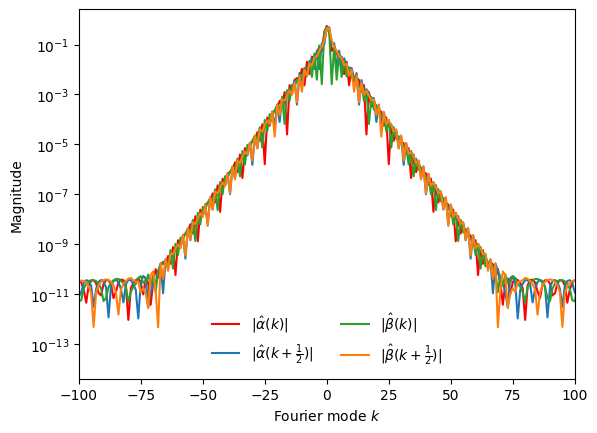
\includegraphics[width=0.3\linewidth]{b6r30eta10.png}
    (b)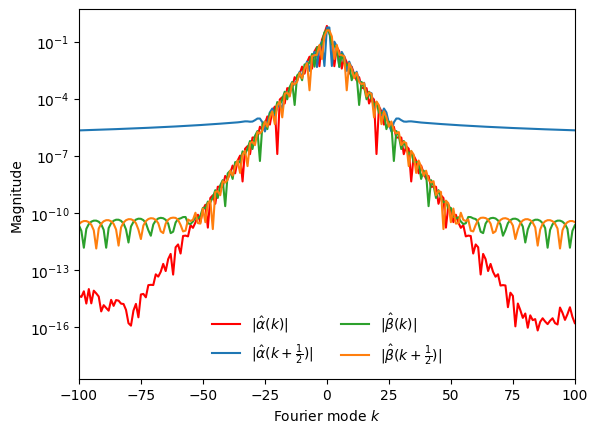
\includegraphics[width=0.3\linewidth]{b6r8eta10.png}
    (c)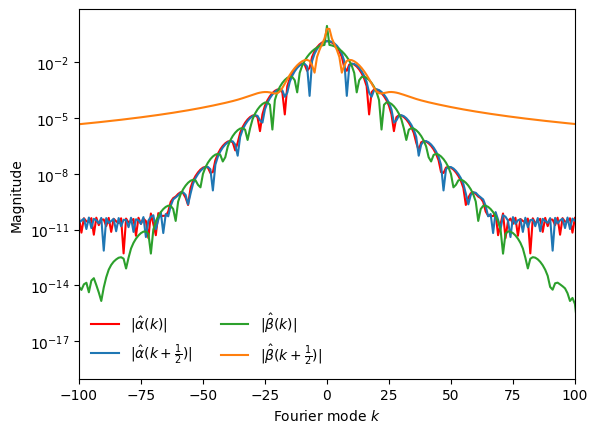
\includegraphics[width=0.3\linewidth]{b1r30eta10.png}
    \caption{Fourier magnitude spectra of the window functions $\hat \alpha(x)$ and $\hat\beta (x)$ sampled on-grid and with a half-grid shift, for (a) $b=6$, $r=30$, $\eta=10$, (b) $b=6$, $r=8$, $\eta=10$, and (c) $b=1$, $r=30$, $\eta=10$.  In each case the spectra exhibit exponential decay near the origin; for the off-grid samples, this eventually crosses over to a algebraic tail. For large enough $r$ and $b$ this crossover point occurs after the machine precision causes a plateau at approximately $10^{-10}$ on most plots.}
    \label{fig:plotwindows}
\end{figure}
\begin{figure}[htbp]
    \centering
    (a)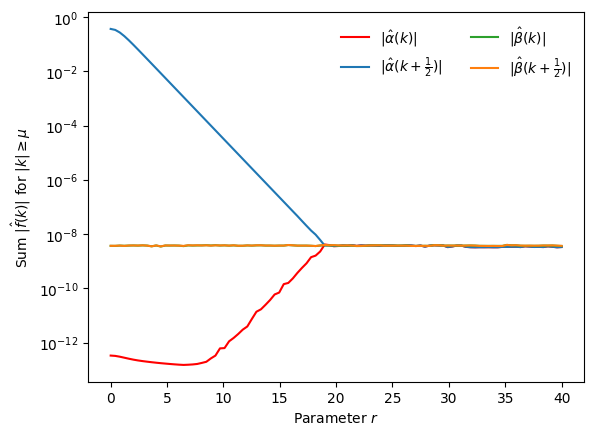
\includegraphics[width=0.3\linewidth]{scalingwithrb6eta10.png}
    (b)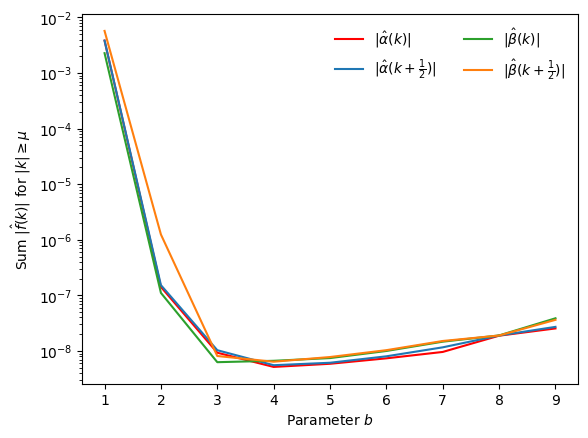
\includegraphics[width=0.3\linewidth]{scalingwithbr1000eta10.png}
    (c)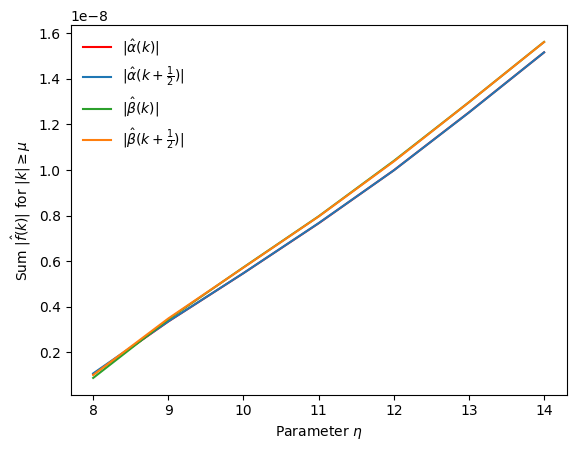
\includegraphics[width=0.3\linewidth]{scalingwithetab6r30.png}
    \caption{Scaling of the $l^1$ norm of Fourier-spectrum magnitude for modes larger than $\mu=100$ for the window functions $\hat \alpha(x)$ and $\hat\beta(x)$, sampled on-grid and with a half-grid shift. (a) Scaling with $r$ for fixed $b=6$ and $\eta=10$; (b) scaling with $b$ for fixed $r=1000$ and $\eta=10$; (c) scaling with $\eta$ for fixed $b=6$ and $r=30$.}
    \label{fig:scaling}
\end{figure}
\begin{figure}[htbp]
    \centering
    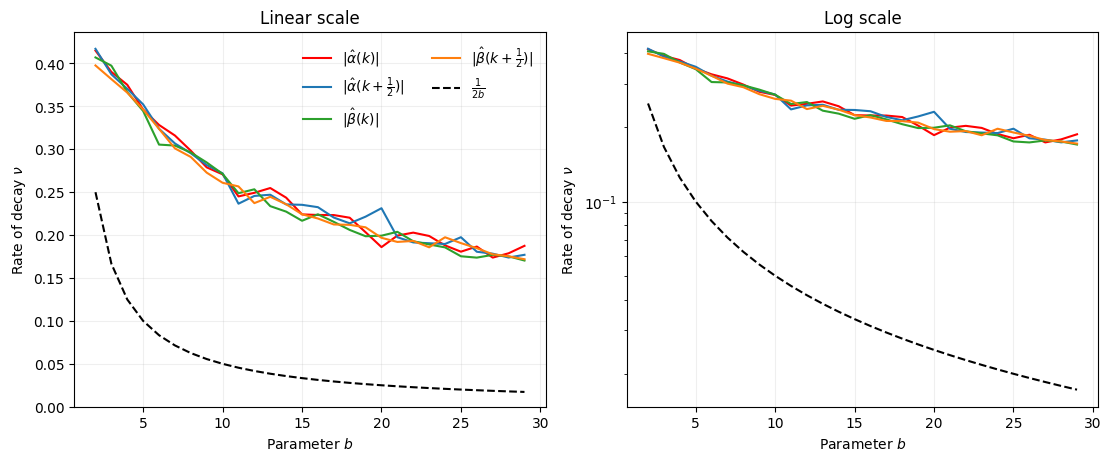
\includegraphics[width=0.75\linewidth]{nur30eta10.png}
    \caption{Scaling of the exponential decay rate $\nu$ of the Fourier-spectrum magnitude with $b$, for fixed $r=30$ and $\eta=10$. The rate is calculated by fitting a line to the log-magnitude spectrum for modes between 0 and 50. Increasing $b$ decreases the rate of exponential decay. It is clear from these plots that the lower bound on $\nu$ we derived is loose.}
    \label{fig:exponent}
\end{figure}
\begin{figure}[htbp]
    \centering
    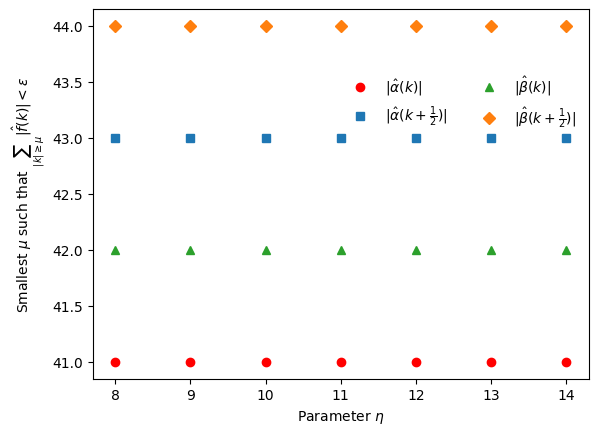
\includegraphics[width=0.4\linewidth]{scalingmuwithetab6r30.png}
    \caption{Smallest bandwidth $\mu$ required to ensure $\sum_{|k|\geq \mu}|f(k)|\leq \epsilon$ plotted against the number of ancilla qubits $\eta$ for $\epsilon = 10^{-6}$, $b=6$, and $r=30$. As expected the smallest bandwidth required for a given $\epsilon$ is independent of $\eta$ for large $r$ and $b$ over the plotted range. }
    \label{fig:scalingmu}
\end{figure}
% \begin{figure}
%     \centering
%     (a)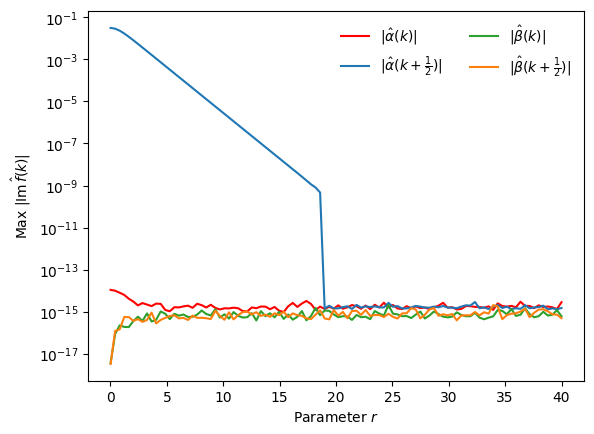
\includegraphics[width=0.4\linewidth]{imscalingwithrb6eta10.png}
%     (b)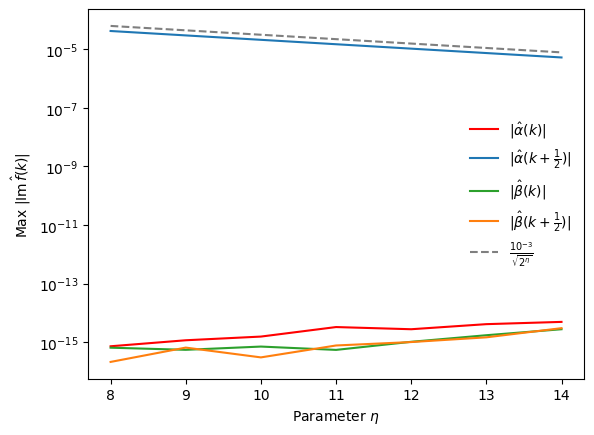
\includegraphics[width=0.4\linewidth]{scalingimwithetab6r6.png}
%     \caption{Scaling of the maximum imaginary part of the Fourier spectra of the window functions $\hat \alpha(x)$ and $\hat\beta(x)$, sampled on-grid and with a half-grid shift. (a) Scaling with $r$ for fixed $b=6$ and $\eta=10$; (b) scaling with $\eta$ for fixed $b=6$ and $r=8$.}
%     \label{fig:imag}
% \end{figure}
\subsection{Conclusion}
We have presented a Boosted State-Independent Quantum Phase Estimation (BSI-QPE) protocol which coherently boosts QPE without requiring a specially prepared input ancilla state. By introducing the window functions via a controlled $R_Y$ rotation on a flag qubit rather than via the input ancilla state, starting from any register value simply translates the output, while the estimation tails remain exponentially suppressed. In doing so we navigate around the no-go theorem of \cite{chen2023quantumthermalstatepreparation}: rather than adding the energy estimate to the register, BSI-QPE shifts the register by approximately the magnitude of the energy, with the sign of this shift recorded in the flag qubit. The only cost of this modification is that any subsequent operation which controls off the value of the energy register must now also control off the flag qubit.

Our construction places unusual demands upon its window functions, requiring a complementary pair satisfying $\alpha(x)^2 + \beta(x)^2 = 1$ with both Fourier transforms decaying exponentially. None of the standard window functions satisfy these requirements, and so we designed a novel pair, $\alpha(x) = \text{sech}( r\cos^{2b} \frac{\pi x}{N})$ and $\beta(x) = \text{tanh}(r \cos^{2b} \frac{\pi x}{N})$. We proved analytically, and confirmed numerically, that their tail weight decays exponentially with the bandwidth $\mu$ for both integer and non-integer energies. This demonstrates that on a quantum computer the best window function is not simply the one with the most concentrated Fourier transform, but the one which also satisfies the constraints imposed by the rest of the quantum algorithm.

BSI-QPE is the key ingredient which allows us to restore the Quantum Metropolis algorithm in Chapter~\ref{chapter:quantum_metropolis}. However, we expect it to find applications in any quantum algorithm which coherently encodes an energy estimate in an ancilla register and then reuses this register without resetting it, as well as in other algorithms which require coherent phase estimation (e.g. HHL \cite{harrow2009quantum}). Finally, our numerics show that the exponential decay rate $\nu$ greatly exceeds our analytical lower bound (Fig.~\ref{fig:exponent}). Tightening this bound, or finding an optimal complementary pair of window functions analogous to the DPSS window, remains an interesting open problem.

\pagebreak
